\chapter{Visualisation algorithms}\label{ch:vis}

One day of one channel is $86400\times100=8.64$ million samples; a screen is a few thousand pixels wide. Every plot of
RS3D therefore \emph{reduces} the data before drawing it. How it is reduced decides whether a short, important spike
survives. This chapter describes the reductions and the geometry of the helicorder.

\section{Reducing a signal for display}
\subsection{Stride decimation and why it can lose a spike}
The simplest reduction keeps every $q$-th sample. It is fast, and for a signal that is oversampled relative to its
bandwidth it is harmless, but for a spiky signal it is wrong: the sampling theorem (Chapter~\ref{ch:data}) applies again,
and a feature narrower than $q$ samples is either kept or discarded depending on where it falls in the grid.
\Cref{fig:minmax} (middle) shows a one-sample spike that stride decimation misses.

\subsection{Min/max decimation}
A seismogram plot is read mainly through its \emph{envelope}, the extremes within each short interval. Min/max
decimation preserves exactly that. The record is divided into $B$ consecutive bins; from each bin the algorithm keeps
the sample with the smallest value and the sample with the largest value (one point if they coincide), in time order.
The plot then has at most $2B$ points and contains the true extremes of every bin:
\begin{equation}\label{eq:minmax}
  \bigl(t^{\min}_b,\,x^{\min}_b\bigr),\ \bigl(t^{\max}_b,\,x^{\max}_b\bigr),\qquad
  x^{\min}_b=\min_{n\in b}x[n],\quad x^{\max}_b=\max_{n\in b}x[n].
\end{equation}
Peak amplitudes and their times are therefore \emph{exact}; what is lost is the detailed shape inside a bin, which
is below the pixel resolution anyway. The cost is linear in the number of samples.

\begin{figure}[tbp]
\centering
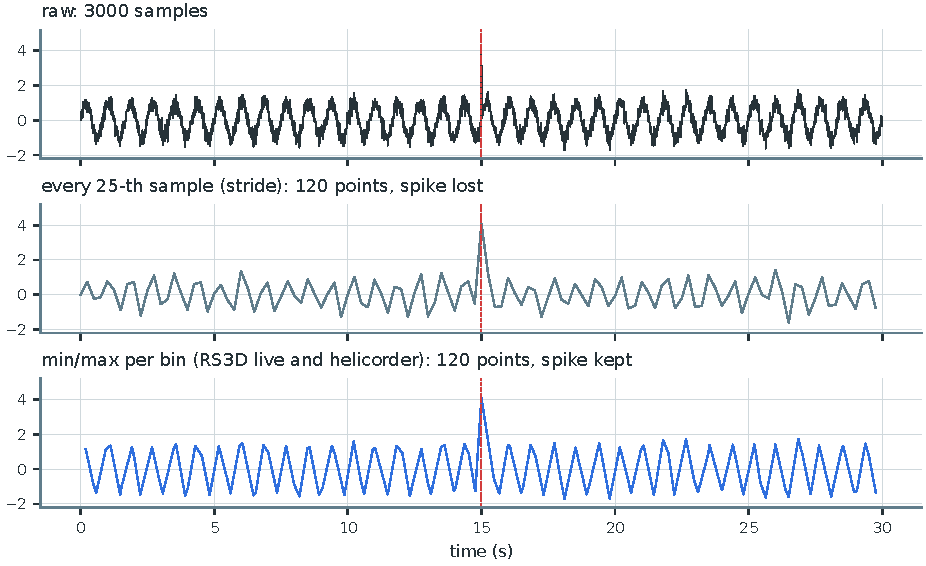
\includegraphics[width=\linewidth]{theory-minmax}
\caption{Reducing 3000 samples to 120 points. Top: the raw signal with one single-sample spike (dashed line).
Middle: every 25th sample, which misses the spike. Bottom: min/max decimation as implemented in
\code{minmax\_decimate}, which keeps it.}\label{fig:minmax}
\end{figure}

\paragraph{Gaps.} The input to the decimator marks gaps with \code{NaN} samples. The record is first split at these
markers, each segment is decimated on its own with a share of the point budget proportional to its length (at least one
bin), and a \code{NaN} is re-inserted between segments, so the plotted line breaks at every gap and no line is drawn
across missing data.

\begin{rs3dapp}
\code{minmax\_decimate(t, v, max\_points)} in \file{core/live.py} is used by the Live view (up to 1500 points per
channel) and by the helicorder (3000 points per row, \code{POINTS\_PER\_ROW}). \textbf{The waveform preview on the Data page
and the detail view are different:} \code{set\_stream\_data} in \file{app/charts.py} thins each trace with a stride of
$\lceil N/4000\rceil$ and then lets the charting library apply its own ``largest-triangle-three-buckets'' downsampling
\parencite{steinarsson2013}, which also preserves visual shape but does not guarantee exact extremes. For the short
windows of the detail view (a few thousand samples) no reduction occurs at all, so the issue arises only for long
previews. Moving the preview to min/max decimation would be a straightforward improvement.
\end{rs3dapp}

\section{The helicorder}
A helicorder (from \emph{helical recorder}) wraps a long record into rows, like lines of text, so that a day fits on one
page and an event stands out as a burst on one line.

\subsection{Geometry}
Let $t_0$ be midnight UTC, $\Delta=1800$~s the row length (30 minutes) and $R=48$ the number of rows. Row $i$ shows the
interval $[t_0+i\Delta,\ t_0+(i+1)\Delta)$. A sample at time $t$ in row $i$ is drawn at horizontal position
\begin{equation}
  x = \frac{t-(t_0+i\Delta)}{60}\quad\text{minutes},\qquad 0\le x<30,
\end{equation}
and vertical position
\begin{equation}\label{eq:heliy}
  y = i - \frac{v(t)-m_i}{S},
\end{equation}
with the $y$ axis pointing down, so a positive excursion moves the trace up. Here $m_i$ is the \emph{median} of row $i$ and
$S$ is a single amplitude scale shared by all rows.

\subsection{Removing the offset}
Raw counts sit on a DC offset (Chapter~\ref{ch:response}). Without $m_i$ the offset divided by $S$ would shift each row
by a fixed fraction of a row, and, worse, would enter the scale $S$ (below), flattening the signal.
\Cref{fig:dcoffset} contrasts the two. The median is used because, unlike the mean, it is not pulled by an earthquake
inside the row.

\begin{figure}[tbp]
\centering
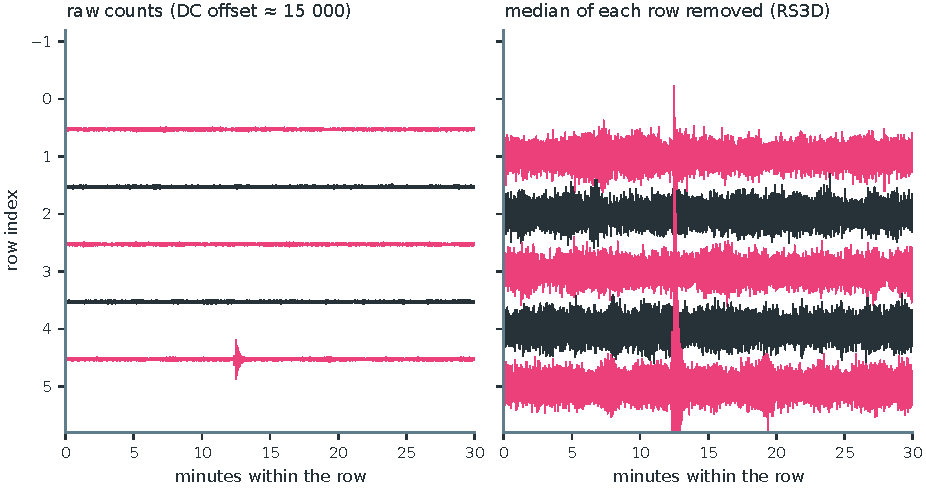
\includegraphics[width=\linewidth]{theory-dc-offset}
\caption{Six rows of the demo EHZ channel with an offset of about 15\,000~counts. Left: raw counts: the offset
dominates the scale and every trace is a nearly flat line shifted by half a row. Right: the median of each row removed:
the signal fills the row height and the small local earthquake is visible in the lower rows.}\label{fig:dcoffset}
\end{figure}

\subsection{The amplitude scale}
The scale $S$ decides how tall the traces are. It must be large enough that adjacent rows do not collide and small
enough that quiet signals are visible. The application sets
\begin{equation}\label{eq:scale}
  S = \frac{2\,P_{99}\bigl(\,\abs{v_{\mathrm{dec}}-m}\,\bigr)}{F},
\end{equation}
where $P_{99}$ is the 99th percentile of the absolute values of all plotted (decimated, median-removed) points of the
day, and $F$ is the user's \ui{Scale} factor ($0.5\times$ to $8\times$). With $F=1$, the 99th percentile maps to half a
row, so ordinary signal fills about one row and only the strongest 1\,\% exceed it. A percentile is used rather than the
maximum so that one huge event does not squash a whole quiet day into flat lines. Note that because the points are min/max
extrema, $P_{99}$ of the decimated data is somewhat larger than that of the raw samples.

\begin{figure}[tbp]
\centering
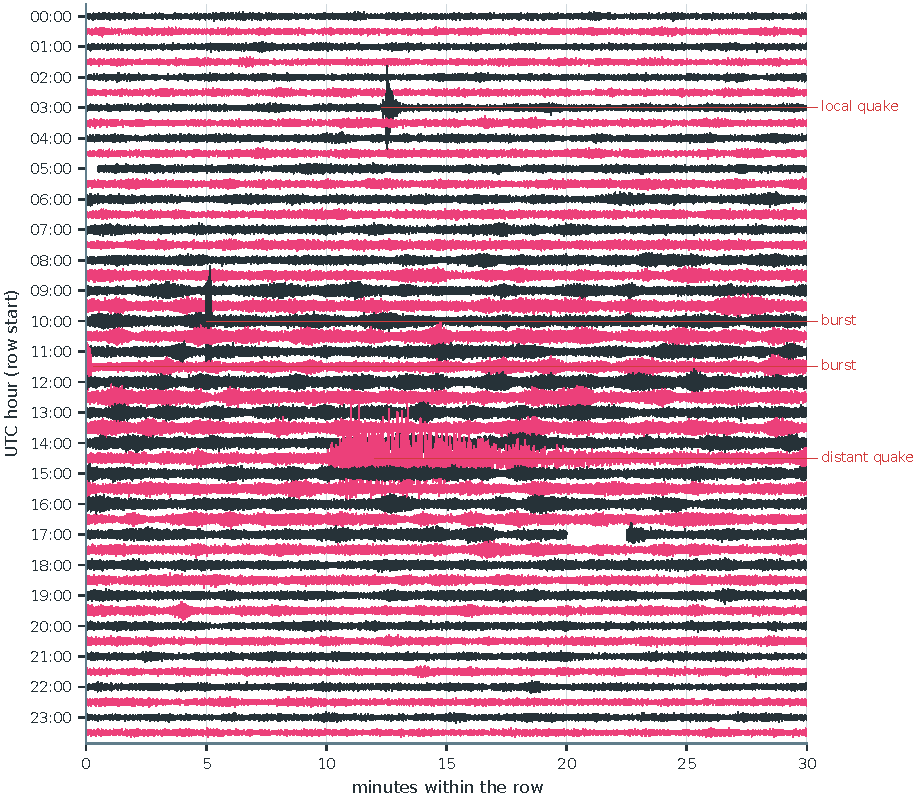
\includegraphics[width=0.92\linewidth]{theory-helicorder}
\caption{A day of the demo EHZ channel drawn with the application's \code{build\_rows} and \code{scale\_for}. Rows are
30~minutes; the day--night change, the local earthquake (03:00 row), two noise bursts, the distant earthquake
(14:30 row) and a gap at 17:20 are visible.}\label{fig:heli}
\end{figure}

\subsection{From a click to a time}
The helicorder page must convert a mouse click into a time. ECharts reports clicks on \emph{data points}, not on empty
space, so the page lays an invisible grid of $48\times180$ points over the plot: one every 10~seconds along each row, drawn as
transparent $10\times14$ pixel rectangles. A click reports the nearest grid point as the pair
$(x_{\min},\,i)$, and the time is
\begin{equation}\label{eq:click}
  t = t_0 + \Delta\left(i + \frac{x_{\min}}{30}\right),\qquad x_{\min}\ \text{clamped to}\ [0,30].
\end{equation}
Equation~\eqref{eq:click} (\code{click\_to\_time} in \file{core/helicorder.py}) is exact for the grid point; the point
itself is at most 5~s from where the pointer was. The chart height is fixed to $48\times14+44$~pixels so that each row is
exactly 14 pixels and a pixel row corresponds to a row index without rounding.

\section{The detail view}
A click opens a window of $T_w=120$~s centred on the clicked time. The toolbar changes this window with a small set of
pure functions (\file{core/helicorder.py}):
\begin{description}[leftmargin=2.4cm,style=nextline]
\item[Zoom out / in] multiplies the span by 2 or $\tfrac12$ about the centre, clamped to between 5 and 3600 seconds.
\item[Earlier / later] shifts the window by $\mp\tfrac12$ of its span.
\item[Box zoom] a dragged rectangle gives a time interval $[x_0,x_1]$ (epoch ms) and an amplitude interval. The new window is
  the rectangle's time span clipped to the current window and widened, centred, to at least 5~s; a rectangle that does not
  overlap the window changes nothing. The amplitude interval, rounded to four significant figures for readable axis
  labels, fixes the vertical axis.
\item[Fit] clears any amplitude zoom, so the axis rescales to the data in view; the time window is kept.
\end{description}

\begin{rs3dkey}
Min/max decimation keeps peaks exact; the helicorder removes each row's median and scales all rows by the same robust
percentile; a click becomes a time through a 10-second grid.
\end{rs3dkey}
